\section{Register File}

\subsection{Overview}
The register file is a fundamental component in the RISC-V processor architecture, responsible for providing fast storage and access to the CPU's general-purpose registers. This module is integral to the CPU's operation, enabling efficient data handling and manipulation during instruction execution.

\subsection{Architectural Design}
A register file consists of a set of registers that can be read and written by specifying the register number. The RISC-V architecture typically uses a register file with 32 registers, each 64 bits wide in the RV64I subset. This allows for rapid data access and storage, crucial for maintaining high performance in processing tasks.

The register file is designed to support multiple read and write operations. Specifically, it includes:
\begin{itemize}
    \item Two read ports, allowing simultaneous reading from two registers.
    \item One write port, enabling the writing of data to a single register per clock cycle.
\end{itemize}

\begin{figure}[h]
\centering
\hspace*{2cm} % Indentation
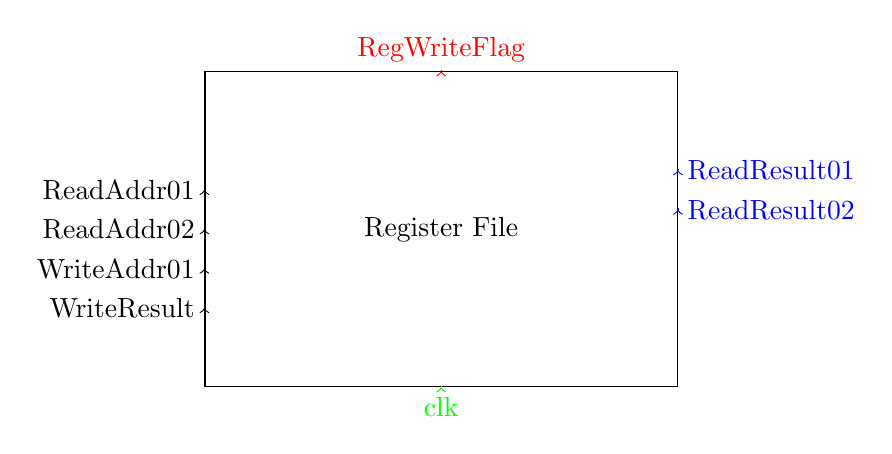
\begin{tikzpicture}
    % Register File Block
    \node[draw, rectangle, minimum width=6cm, minimum height=4cm] (regfile) {Register File};

    % Inputs
    \node[anchor=south, text=red] (regwrite) at (regfile.north) {RegWriteFlag};
    \node[anchor=east] (readaddr1) at (regfile.west |- 1, 0.5) {ReadAddr01};
    \node[anchor=east] (readaddr2) at (regfile.west |- 2, 0) {ReadAddr02};
    \node[anchor=east] (writeaddr) at (regfile.west |- 3, -0.5) {WriteAddr01};
    \node[anchor=east] (writeresult) at (regfile.west |- 4, -1) {WriteResult};
    \node[anchor=north, text=green] (clk) at (regfile.south) {clk};

    % Outputs
    \node[anchor=west, text=blue] (readresult1) at (regfile.east |- 1, 0.75) {ReadResult01};
    \node[anchor=west, text=blue] (readresult2) at (regfile.east |- 2, 0.25) {ReadResult02};

    % Arrows
    \draw[->, red] (regwrite.south) -- (regfile.north);
    \draw[->] (readaddr1.east) -- (regfile.west |- 1, 0.5);
    \draw[->] (readaddr2.east) -- (regfile.west |- 2, 0);
    \draw[->] (writeaddr.east) -- (regfile.west |- 3, -0.5);
    \draw[->] (writeresult.east) -- (regfile.west |- 4, -1);
    \draw[->, green] (clk.north) -- (regfile.south);
    \draw[->, blue] (regfile.east |- 1, 0.75) -- (readresult1.west);
    \draw[->, blue] (regfile.east |- 2, 0.25) -- (readresult2.west);
\end{tikzpicture}
\caption{Register File Block Diagram}
\end{figure}

\subsection{Functional Operation}
In the context of the RISC-V CPU, the register file interacts closely with other components such as the ALU (Arithmetic Logic Unit) and instruction decoder. During the execution of R-format instructions, for example, the register file provides the operands for the ALU and stores the result of the computation.

The typical operations involving the register file include:
\begin{enumerate}
    \item \textbf{Read Operations}: Two source registers are read, and their values are provided to the ALU or other computational units.
    \item \textbf{Write Operations}: The result of an ALU operation or a value loaded from memory is written back to a destination register.
\end{enumerate}

The design ensures that reads are combinational operations, meaning the data is immediately available based on the provided register addresses. Writes, however, are sequential operations controlled by a clock signal to ensure data integrity and proper synchronization.

\subsection{Integration with CPU Architecture}
The register file is crucial for the overall performance of the CPU as it stores the operands and results of arithmetic and logic operations. It interfaces directly with the instruction memory, instruction decoder, and the ALU:
\begin{itemize}
    \item \textbf{Instruction Memory}: The instruction memory fetches instructions that specify which registers to read from and write to.
    \item \textbf{Instruction Decoder}: The decoder interprets the instructions and generates control signals required to access the register file.
    \item \textbf{ALU}: The ALU performs computations using the data read from the register file and stores the results back into the register file.
\end{itemize}

\begin{figure}[h]
\centering
\hspace*{2cm} % Indentation
\begin{tikzpicture}
    % Blocks
    \node[draw, rectangle, minimum width=3cm, minimum height=1.5cm] (instmem) {Instruction Memory};
    \node[draw, rectangle, minimum width=3cm, minimum height=1.5cm, below=1cm of instmem] (instdec) {Instruction Decoder};
    \node[draw, rectangle, minimum width=3cm, minimum height=1.5cm, below=1cm of instdec] (regfile) {Register File};
    \node[draw, rectangle, minimum width=3cm, minimum height=1.5cm, below=1cm of regfile] (alu) {ALU};
    \node[draw, rectangle, minimum width=3cm, minimum height=1.5cm, right=4cm of regfile] (datamem) {Data Memory};

    % Arrows
    \draw[->] (instmem.south) -- (instdec.north);
    \draw[->] (instdec.south) -- (regfile.north);
    \draw[->] (regfile.south) -- (alu.north);
    \draw[<->] (alu.east) -- (datamem.west);
    \draw[->] (alu.west) -- ++(-1,0) node[midway, above] {Result} -- ++(0,2.5) -- (regfile.west);

\end{tikzpicture}
\caption{Integration of Register File within the CPU}
\end{figure}

\subsection{Initialization and Read/Write Synchronization}
In practical implementations, some registers in the register file may be initialized to specific values for various purposes, such as testing or specific algorithmic requirements. This initialization can be crucial for certain applications or during the boot process of the CPU.

The read operations are usually instantaneous, providing the required data to the ALU or other processing units without delay. Write operations are synchronized with the clock to ensure data integrity and prevent race conditions.

\subsection{Signal Descriptions}
The key signals associated with the register file include:
\begin{itemize}
    \item \textbf{clk}: The clock signal that synchronizes the write operations.
    \item \textbf{regWriteFlag}: A control signal indicating whether a write operation should be performed.
    \item \textbf{readAddr01, readAddr02}: Addresses of the registers to be read.
    \item \textbf{writeAddr01}: Address of the register to be written.
    \item \textbf{writeResult}: Data to be written to the specified register.
    \item \textbf{readResult01, readResult02}: Data read from the specified registers.
\end{itemize}

\subsection{Conclusion}
The register file is a crucial part of the RISC-V processor, enabling efficient and fast access to frequently used data. Its design supports simultaneous reads and controlled writes, ensuring high performance and reliability. Understanding the operation and integration of the register file within the processor architecture is essential for implementing and optimizing RISC-V systems.

